% -----------------------------------------------------------------------------
% ########################
% # PREDLOGA ZA POROCILO #
% ########################
%
% @author Iztok Starc
% @date   3. december 2008
%
\documentclass[a4paper,12pt]{report}

% -----------------------------------------------------------------------------
% ####################################################
% # UPORABA PAKETOV - NASTAVITEV JEZIKA in KODIRANJA #
% ####################################################
\usepackage[slovene]{babel}
\usepackage[utf8]{inputenc}
\usepackage{lmodern}
\usepackage[T1]{fontenc}
\usepackage{iwona}

% -----------------------------------------------------------------------------
% ######################################
% # VNOS KLJUCNIH PARAMETROV BESEDILA  #
% ######################################

\newcommand{\naslov}     {Cake Shop}
\newcommand{\prviavtor}  {Aleš Matijevič}
\newcommand{\prviindeks} {63000214}
\newcommand{\drugiavtor} {Igor Jončevski}
\newcommand{\drugiindeks}{63070420}
\newcommand{\tretjiavtor}{Mia Erbus}
\newcommand{\tretjiindeks}{63050184}
\newcommand{\kraj}       {Ljubljana}

% -----------------------------------------------------------------------------
% ###################
% # UPORABA PAKETOV #
% ###################
\usepackage[a4paper,left=25mm,right=25mm,top=20mm,bottom=30mm,includehead]{geometry}

\usepackage{graphicx, epsfig}

\usepackage{fancyhdr}

\usepackage[
colorlinks=true, linkcolor=blue, citecolor=red,
%
pdftitle={\naslov},
pdfauthor={\prviavtor, \drugiavtor},
pdfsubject={Poročilo seminarske naloge pri predmetu Elektronsko Poslovanje},
pdfkeywords={spletna prodajalna, PHP, SSL, MySQL}, a4paper, pagebackref=true, unicode]{hyperref}

% -----------------------------------------------------------------------------
\begin{document}

% -----------------------------------------------------------------------------
% ##################
% # NASLOVNA STRAN #
% ##################
\begin{titlepage}
	\begin{center}
	{UNIVERZA V LJUBLJANI\\[10pt] 
	FAKULTETA ZA RAČUNALNIŠTVO IN INFORMATIKO}

	\vspace{65mm}

	{\Large\textbf{\naslov}}

	\vspace{10mm}

	{\large Poročilo seminarske naloge pri predmetu\\[10pt] Elektronsko poslovanje}

	\vfill
	\vspace{60mm}

\hspace{20mm}
\begin{minipage}[t]{70mm}
	{\bf Študenti}\\
	{\prviavtor} ({\prviindeks})\\ 
	{\drugiavtor} ({\drugiindeks})\\
	{\tretjiavtor} ({\tretjiindeks})
\end{minipage}
%\hfill
\begin{minipage}[t]{50mm}
	{\bf Mentor}\\
	David Jelenc
\end{minipage}
%\hspace{20mm}

	\vspace{40mm}

	{	\kraj, \today}
	\end{center}
\end{titlepage}

% -----------------------------------------------------------------------------
% ##################
% # KAZALO VSEBINE #
% ##################

\tableofcontents
% -----------------------------------------------------------------------------
% ############
% # POVZETEK #
% ############
\begin{abstract}
Pri predmetu Elektronsko poslovanje smo morali kot seminarsko nalogo izdelati spletno prodajalno. Ker smo za osnovo izbrali CakePHP ogrodje za izdelavo spletnih aplikacij, smo tudi spletno prodajalno poimenovali cakeshop. CakeShop je torej ime naše spletne prodajalne in dejansko predstavlja prodajalno slaščic oz. različnih tort. Podatke in slike o tortah smo na avtomatiziran način pridobili iz različnih internetnih virov, v večini pa iz Wikipedije. Skratka izdelali smo aplikacijo za prodajo tort. 
\end{abstract}

% -----------------------------------------------------------------------------
% ##################
% # UVOD DOKUMENTA #
% ##################
\chapter{Uvod}

%{\it V uvodu podajte kratko in jedrnato predstavitev teme seminarske naloge, navedite seznam uporabljene tehnologije ter naštejte uporabljene mehanizme za nadzor dostopa.}

Izdelali smo aplikacijo CakeShop, namenjeno prodajalcem in kupcem tort.

\section{Uporaba tehnologij}

Pri izdelavi smo uporabili tehnologije:

\begin{itemize}
  \item Skritni jezik PHP.
  \item Ogrodje za izdelavo spletnih aplikacij, CakePHP.
  \item Poizvedbeni jezik SQL.
  \item Sistem za upravljanje s podatkovno bazo MySQL.
  \item Spletni strežnik Apache2.
  \item Programski vzorec MVC (Model View Controller).
  \item Koncept obdelave zahtev REST.
  \item Koncept oblikovanja in dostopa do podatkovne baza (ORM).
  \item Koncept zapisovnanja in CRUD.
  \item Stiliranje z uporabo CSS.
  \item Skriptni jezik javascript.
  \item GitHub za izmenjavo datotek med člani skupine.
\end{itemize}

\section{Mehanizmi za nadzor dostopa}

Mehanizmi za nadzor dostopa:
\begin{itemize}
  \item SSL/TLS/HTTPS.
  \item ACL (access control list).
  \item Preverjanje avtentičnosti v podatkovni bazi z uporabniškim imenom in geslom, generiranim z zgoščevalno funkcijo.
  \item Preverjanje avtentičnosti strežnika z digitalnim potrdilom.
\end{itemize}

% -----------------------------------------------------------------------------
% ###################
% # JEDRO DOKUMENTA #
% ###################

% -----------------------------------------------
\chapter{Primeri uporabe}

%{\it Kratek in jedrnat opis vlog uporabnikov ter funkcionalnosti, ki so vsaki vlogi dostopne. Če ste implementirali funkcionalnosti, ki se točkujejo z dodatnimi točkami, jih posebej izpostavite.}

Ustvarili smo tri vloge uporabnikov:
\begin{enumerate}
  \item Stranka
  \item Prodajalec
  \item Administrator
\end{enumerate}

\section{Anonimni uporabnik}

Vsak anonimni oz. neprijavljeni obiskovalec strani lahko brska med tortami, ki so opremljene s slikami. Implementirali smo tudi funkcijo iskanja tort s celotnimi ali delnimi ključnimi besedami. Anonimni uporabnik ima možnost registracije uporabniškega imena in prijave.

\section{Stranka}

Ko se anonimni uporabnik prijavi, postane prijavljen uporabnik oz. stranka. Podobno kot anonimni uporabnik, tudi stranka lahko brska med izdelki. Ko se odloči za nakup izdelka, se izdelek doda v košarico. V košarici lahko določi, koliko primerkov tega izdelka želi. V primeru, da si premisli, lahko izdelek izbriše iz košarice. Ko je stranka zadovoljna z izborom izdelkov, košarico pošlje na blagajno (check-out).

\begin{figure}[htb]
	\centering
	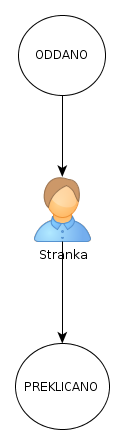
\includegraphics[width=2.5cm]{img/shema1.png}
	\caption{Možna stanja stranke}
\label{fig:1}
\end{figure}

\section{Prodajalec}

Prodajalec ima možnost dodajanja izdelkov, kjer določi atribute: ime, opis, cena, količna in vidnost. Izdelke lahko naknadno uredi in naloži nove slike ali izbriše že obstoječe. Možno jih je tudi izbrisati. Ima tudi možnost urejanja naročil. Pri vsakem naročilu lahko pregleda njegove podrobnosti. Naročilu lahko spremeni stanje. Glede na stanje, v katerem je naročilo, se mu ponudijo vsa možna naslednja stanja. Ima tudi možnost dodajanja in urejanja strank.

\begin{figure}[htb]
	\centering
	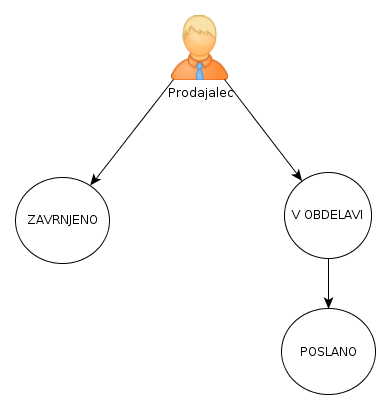
\includegraphics[width=8.5cm]{img/shema2.png}
	\caption{Možna stanja prodajalca}
\label{fig:1}
\end{figure}

\section{Administrator}

Administrator ima možnost dodajanja in urejanja prodajalcev ter strank. Vloga administratorja je ključna saj poleg omenjenih akcij lahko izbrane prodajalce tudi deaktivira oz. aktivira. V ta namen smo razvili tudi poseben seznam, na katerem so vidni deaktivirani uporabniki in ima administrator možnost jih spet aktivirati.

\section{Dodatne funkcionalnosti}

Implementirali smo tudi nekaj dodatnih funkcij, in sicer:

\begin{itemize}
  \item iskanje izdelkov,
  \item razdelitev prikaza izdelkov na posamezne strani (paginacija),
  \item sortiranje izdelkov po ceni in nazivu,
  \item predstavitev izdelkov s slikami in
  \item stiliziranje aplikacije s CSS predlogami.
\end{itemize}

Iskanje deluje z uporabo SQL pogoja LIKE po poljih naslov in opis izdelka, tak način iskanja omogoča uporabniku, da najde vse željene izdelke.

Za preglednejši pogled nad izdelki smo s pomočjo CakePHP funkcije implementirali paginacijo nad izdelki. Stranke in prodajalci lahko brskajo med izdelki tako, da se s kliki pomikajo naprej in nazaj.

Uporabnik si iskalne rezultate lahko uredi oz. sortiranje po ceni in nazivu samega izdelka. Tako lahko uporabnik pridobi najbolj poceni oz. najdražje izdelke.

V podatkovni bazi smo dodali tabelo slik. Vsak izdelek je lahko predstavljen brez slike (v tem primeru se mu dodeli privzeta slika), lahko pa z večimi slikami, od katerih je samo ena prikazna slika. Uporabnik z vlogo prodajalec lahko preko priočnega vmesnika naloži sliko izdelka s svojega računalnika.

Dodali smo tudi CSS predloge, ki naredijo spletno prodajalno bolj prijazno za uporabnikove oči in ga tako bolj nagovori k nakupu izdelkov v naši spletni prodajalni.
% -----------------------------------------------
\chapter{Uporabniške pristopne točke}

%{\it Opis uporabniških pristopnih točk. Tukaj lahko dokumentirate uporabniški vmesnik za ključne primere uporabe, tako da zajamete zaslonske slike vaše aplikacije in jih opremite s komentarji.}

\section{Prijava}

Ko se uporabnik želi prijaviti v sistem, mu ponudimo vnos uporabniškega imena in gesla.

\begin{figure}[htb]
	\centering
	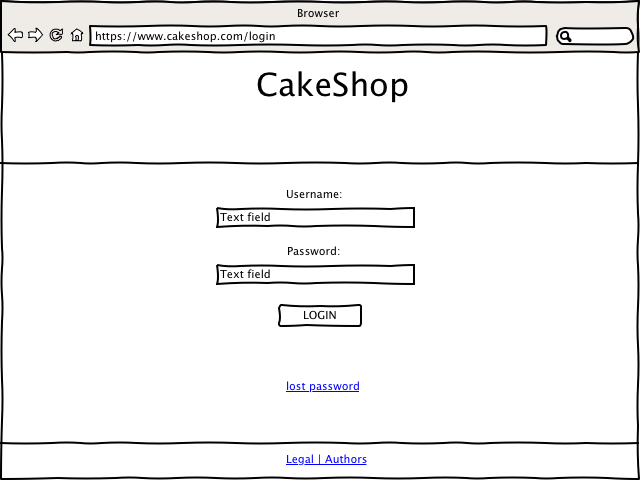
\includegraphics[width=13cm]{Wireframes/cakeshop/pngs/010200-LoginAnonymous.png}
	\caption{Prijava}
\label{fig:1}
\end{figure}

\newpage

\section{Prikaz izdelkov}

Uporabnik se je prijavil v sistem in v bazi je njegovo uporabniško ime zabeleženo kot stranka. Prikažemo mu vse izdelke v bazi, skupaj s slikami. Izdelke lahko gledamo s paginacijo. Na vsaki strani se jih prikaže določeno število. Omogočeno je tudi sortiranje po imenu (po abecedi) ali po ceni.

\begin{figure}[htb]
	\centering
	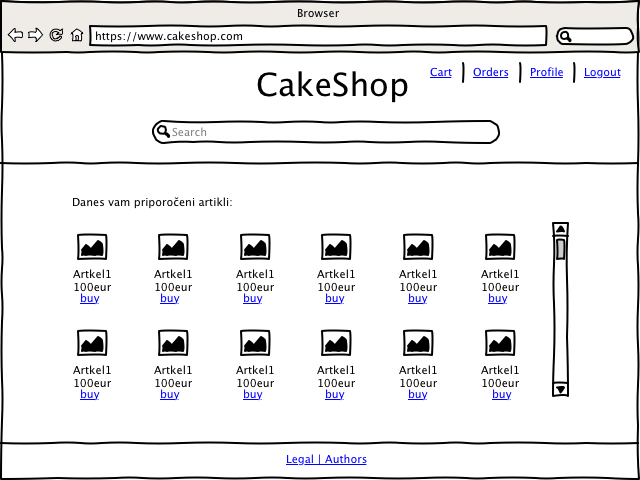
\includegraphics[width=13cm]{Wireframes/cakeshop/pngs/020000-IndexClient.png}
	\caption{Košarica}
\label{fig:2}
\end{figure}

\section{Podrobnosti izdelka}

Ko stranka izbere določen izdelek, ki ga želi kupiti, klikne na gumb "buy". V tem koraku se izdelek doda v košarico.

\begin{figure}[htb]
	\centering
	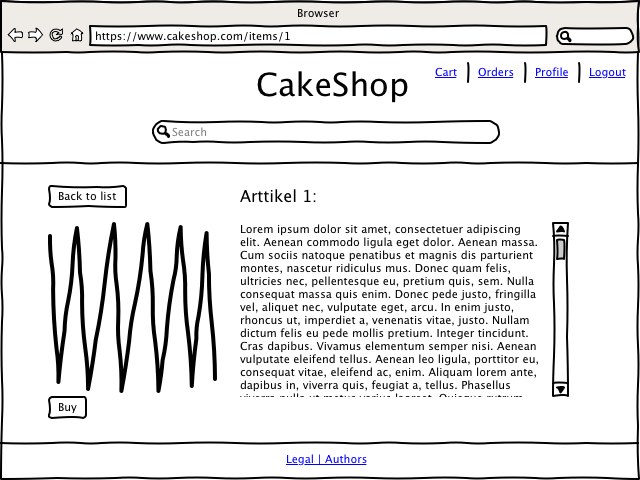
\includegraphics[width=13cm]{Wireframes/cakeshop/pngs/020100-ItemsDetailsClient.png}
	\caption{Podrobnosti izdelka}
\label{fig:3}
\end{figure}

\section{Dodajanje v košarico}

V košarici so navedeni vsi izdelki, ki jih stranka želi kupiti. Stranka lahko izdelke uredi, tako da navede poljubno količino posameznega izdelka. Če izdelka ne želi, ga lahko iz košarice izbriše.

\begin{figure}[htb]
	\centering
	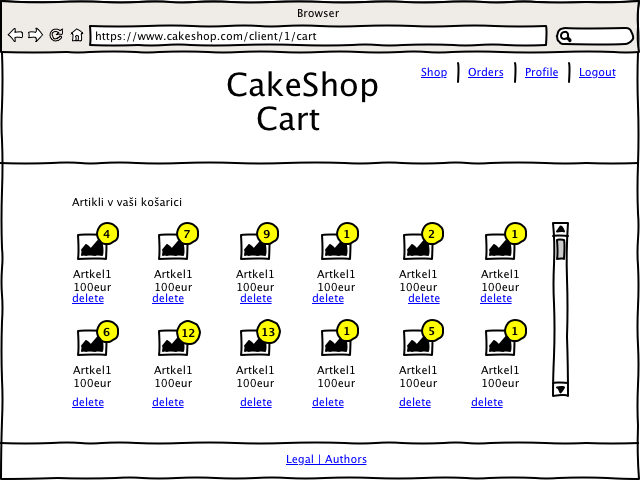
\includegraphics[width=13cm]{Wireframes/cakeshop/pngs/020200-CartViewClient.png}
	\caption{}
\label{fig:4}
\end{figure}

\section{Blagajna}

Na blagajni lahko stranka preglejuje svoja naročila. Vidi pa tudi status svojega naročila. Status je lahko v več stanjih:

\begin{itemize}
  \item {\it oddano}: stranka odda naročilo,
  \item {\it preklicano}: stranka prekliče svoje naročilo,
  \item {\it v obdelavi}: prodajalec sprejme naročilo,
  \item {\it zavrnjeno}: prodajalec prekliče naročilo,
  \item {\it poslano}: prodajalec odda naročilo.
\end{itemize}

Naročila lahko tudi sortiramo po vseh stolpcih.

\begin{figure}[htb]
	\centering
	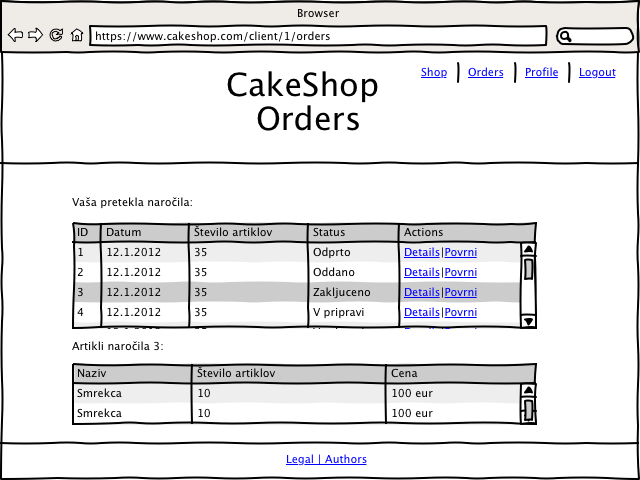
\includegraphics[width=13cm]{Wireframes/cakeshop/pngs/020300-OrdersViewClient.png}
	\caption{Blagajna}
\label{fig:5}
\end{figure}

\section{Prodajalec}

Prodajalec ima možnost urejanja izdelkov. Naloži lahko poljubno sliko izdelka, spremeni ime in opis izdelka.

\begin{figure}[htb]
	\centering
	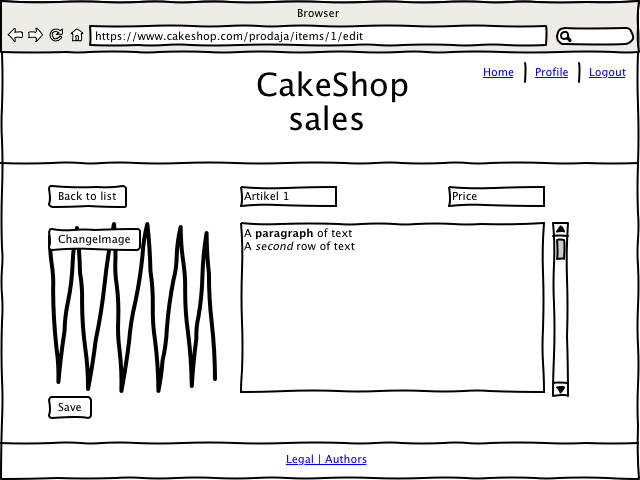
\includegraphics[width=13cm]{Wireframes/cakeshop/pngs/030101-ItemsDetailsSalesman.png}
	\caption{Prodajalec}
\label{fig:5}
\end{figure}

\section{Urejanje profila}

Stranka ima možnost urejanja svojega profila. Prodajalec ima možnost urejanja svojega profila in profile strank. Administrator ima možnost urejanja vseh profilov.

\begin{figure}[htb]
	\centering
	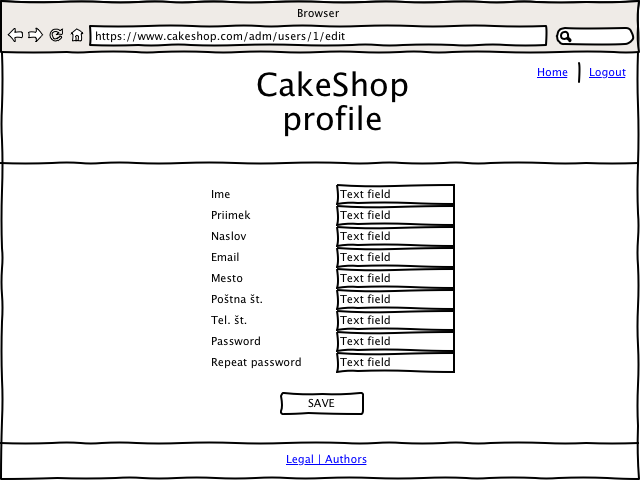
\includegraphics[width=13cm]{Wireframes/cakeshop/pngs/040201-ProfileClientsAdmin.png}
	\caption{Prodajalec}
\label{fig:5}
\end{figure}


% -----------------------------------------------
\chapter{Podatkovni model}

%{\it Slika logičnega podatkovnega modela (denimo iz programa MySQL Workbench) ter kratek opis tabel in obrazložitev netrivialnih atributov.}

Podatkovno bazo smo predstavili s šestimi tabelami. V tabeli {\bfseries users} smo navedli atribute uporabnika. Zanimiva sta atributa {\it post id}, ki se navezuje na tabelo {\bfseries posts}, v kateri so shranjene pošte krajev, in {\it active}, ki označuje, ali gre za aktiviranega ali neaktiviranega uporabnika. Vsak uporabnik lahko naroči več naročil, vsako naročilo pripada enemu uporabniku. Uporabnik živi v eni pošti, v pošti lahko živi več uporabnikov.

Tabela {\bfseries items orders} je povezovalna tabela med izdelki in naročili. Preko atributa {\it order id} dobimo povezavo na tabelo {\bfseries orders}. Preko atributa {\it item id} dobimo povezavo na tabelo {\bfseries items} in s tem vse izdelke, ki so v posameznem naročilu.

Tabela {\bfseries images} se preko atributa {\it item id} navezuje na tabelo {\bfseries items}. Povezava med njima je 1:n, kar pomeni, da ima lahko izdelek več slik, vsaka slika pa pripada enemu izdelku.

\begin{figure}[htb]
	\centering
	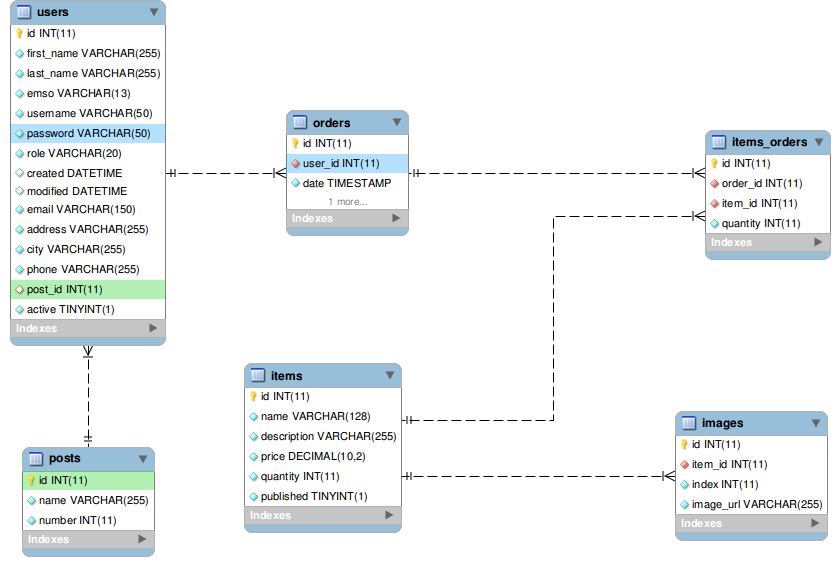
\includegraphics[width=13cm]{img/ER-model.png}
	\caption{ER model}
\label{fig:4}
\end{figure}


% -----------------------------------------------
\chapter{Varnost sistema}

%{\it Opis mehanizmov nadzora dostopa in ostalih varnostnih mehanizmov implementacije (SSL/TLS, preverjanje vnosov odjemalca, CAPTCHA, uporaba regularnih izrazov, \dots).}

Za zagotavljanje varnosti spletne prodajalne smo uporabili protokol HTTPS, ki temelji na tehnologiji SSL/TLS, ki zagotavlja tajnost prenosa podatkov. Tak način zagotavljanja varnosti uporablja princip javnih in privatnih ključev. V trenutku, ko se klient poveže na strežnik, se prenese javni ključ strežnika. Vsa komunikacija med strežnikom in klientom je na tej stopnji kriptirana s pomočjo javnega ključa strežnika. Na tak način se zagotovi identifikacija strežnika in tajnost prenešenih informacij. 

V seminarski nalogi smo uporabljali samopodpisano digitalno potrdilo strežnika, kar je primerno le v testne namene. V dejanski produkcijski verziji bi morali uporabiti overjeno digitalno potrdilo s strani agencije za overjanje digitalnih potrdil npr. SI-GENCA. Le na podlagi tako overjenega digitalnega potrdila lahko stranke zaupajo identiteti, ki jo izraža javni ključ.       

Določeni deli prodajalne so vzpostavljeni tudi preko nezavarovanega kanala in tako omogočajo anonimnemu odjemalcu pregled in ogled artiklov. Vsi ostali deli spletne prodajalne oz. trgovine pa s strežnikom komunicirajo preko zavarovanega kanala. Prehajanje med zavarovanim in nezavarovanim kanalom smo implementirali v sami aplikaciji z uporabo php SERVER spremnljivke in nekaj if stavki. Tako smo dosegli da je za nekatere dele naprimer registracija oz. prijava uporabnika nujno potrebna uporaba varnega kanala.

% -----------------------------------------------
\chapter{Izjava o avtorstvu seminarske naloge}

Spodaj podpisani \textit{\prviavtor}, vpisna številka \textit{\prviindeks}, sem (so)avtor seminarske naloge z naslovom \textit{\naslov}. S svojim podpisom zagotavljam, da sem izdelal ali bil soudeležen pri izdelavi naslednjih sklopov seminarske naloge:
\begin{itemize}
    \item Vzpostavitev ogrodja CakePHP
	\item Vzpostavitev SSL modeula
	\item Izdelava kontorlerjev aplikacije
\end{itemize}

Podpis: {\prviavtor}, l.r.

\newpage

Spodaj podpisani \textit{\drugiavtor}, vpisna številka \textit{\drugiindeks}, sem (so)avtor seminarske naloge z naslovom \textit{\naslov}. S svojim podpisom zagotavljam, da sem izdelal ali bil soudeležen pri izdelavi naslednjih sklopov seminarske naloge:
\begin{itemize}
    \item Baza
    \item Naročila
    \item Vzpostavitev ogrodja CakePHP
\end{itemize}

Podpis: {\drugiavtor}, l.r.

\newpage

Spodaj podpisana \textit{\tretjiavtor}, vpisna številka \textit{\tretjiindeks}, sem (so)avtor seminarske naloge z naslovom \textit{\naslov}. S svojim podpisom zagotavljam, da sem izdelal ali bil soudeležen pri izdelavi naslednjih sklopov seminarske naloge:
\begin{itemize}
	\item Shema ER modela
    \item Vzpostavitev ogrodja CakePHP
    \item Priprava skic aplikacije
    \item Priprava primerov uporabe
    \item Testiranje in beleženje napak
\end{itemize}

Podpis: {\tretjiavtor}, l.r.

 -----------------------------------------------------------------------------
% #######################
% # ZAKLJUCEK DOKUMENTA #
% #######################
\chapter{Zaključek}

K izdelavi aplikacije smo v začetku pristopili organizirano oz. projektno in začeli s fazo izdelave primerov uporabe. Nadaljevali smo z izdelavo skic aplikacije. Te dve aktivnosti so nas pripeljale do jasne slike podatkovne baze in sistemske ureditve same aplikacije. Sledila je faza izbire ogrodja za izdelavo spletnih aplikaicj, kjer smo upoštevali različne parametre in izbirali med različnimi kanditati. Ko je bilo ogrodje izbrano smo identificirali naloge in te naloge razdelili med člane skupine. Sledila je faza dejanskega razvoja in priprave aplikacije. Med samo izdelavo aplikacije smo spoznali različne uporabne tehnologije, s katerimi smo podprli različne aspekte spletne prodajalne. 

% -----------------------------------------------------------------------------
% ##############
% # LITERATURA #
% ##############
\begin{thebibliography}{99}
\addtocounter{chapter}{1}
\addcontentsline{toc}{chapter}{\protect\numberline{\thechapter}Literatura}
\addtocontents{toc}{\protect\vspace{15pt}}

\bibitem{bib:ref} Starc I. \emph{Študijsko gradivo za laboratorijske vaje predmeta Elektronsko poslovanje}

\bibitem{bib:IPsecHowTo1} CakePHP dokumentacija. 2011. (citirano \today). Dostopno na naslovu:
\url{http://book.cakephp.org/2.0/en/}


\end{thebibliography}

% -----------------------------------------------------------------------------
% ###########
% # DODATEK #
% ###########

%\appendix

%\chapter{Naslov dodatka}
%{\it Po potrebi.}

\end{document}
